\section{Results and Discussion}

\begin{figure}%[!htbp]

\begin{center}
\setlength\tabcolsep{1.5pt} % default value: 6pt
\medmuskip=-2mu
\thinmuskip=-2mu
\thickmuskip=-2mu
\nulldelimiterspace=-1pt
\scriptspace=0pt
\begin{tabular}{ | c || c c c | c c c | }
  \multicolumn{1}{c}{} & \multicolumn{3}{c}{Competitors} & \multicolumn{3}{c}{Mean Dominant ($\pm S.D.$)} \\
 \cline{2-7}
  \multicolumn{1}{c|}{} & \tiny{$P_{1} = 1.0$} & \tiny{$P_{2} = P_{1}$} & \tiny{$P_{2} > P_{1}$} & \tiny{$P_{1} = 1.0$} & \tiny{$1.0 > P_{1} > P_{2}$} & \tiny{$P_{2} \geq P_{1}$}  \\
 \hline
 $n$ & 1 & 1 & 1 & 9 & 7 & 34  \\
 \hhline{|=||===|===|}
 $A_1$ & 0.00 & 1.00 & 1.00 & $0.23 \pm 0.35$ & $0.50 \pm 0.47$ & $0.57 \pm 0.46$ \\
 $A_2$ & 1.00 & 0.91 & 1.00 & $1.00 \pm  0.00$ & $1.00 \pm 0.00$ & $1.00 \pm 0.00$ \\
 \hline
 $P_{c}$ & 0.85 & 0.00 & 0.00 & $0.00 \pm 0.00$ & $0.00 \pm 0.00$ & $0.03 \pm 0.05$ \\
 $P_1$ & 0.07 & 1.00 & 0.00 & $1.00 \pm 0.00$ & $0.60 \pm 0.07$ & $0.28 \pm 0.16$ \\
 $P_2$ & 0.08 & 0.00 & 1.00 & $0.00 \pm 0.00$ & $0.40 \pm 007$ & $0.69 \pm 0.14$ \\
 \hline
 $C_1$ & 21.8 & 7.2 & 9.9 & $3.90 \pm 0.60$ & $3.38 \pm 0.33$ & $3.03 \pm 0.69$ \\
 $C_2$ & 101.2 & 274.2 & 238.2 & $230.6 \pm 71.1$ & $192.7 \pm 45.3$ & $271.6 \pm 73.6 $ \\
 \hline
 $E_{c}$ & 0.21 & 0.00 & 0.00 & $0.29 \pm 0.37$ & $0.44 \pm 0.59$ & $0.21 \pm 0.75$ \\
 $E_1$ & 1.21 & 30.1 & 0.00 & $47.2 \pm 21.7$ & $21.3 \pm 12.0$ & $4.62 \pm 7.05$ \\
 $E_2$ & 2.49 & 54.1 & 38.8 & $231.2 \pm 94.3$ & $283.1 \pm 57.0$ & $325.4 \pm 68.9$ \\
 \hline
 $M_{c}$ & 0.53 & 0.30 & 0.90 & $0.33 \pm 0.41$ & $0.74 \pm 0.31$ & $0.67 \pm 0.35$ \\
 $M_1$ & 1.00 & 0.00 & 1.00 & $0.52 \pm 0.41$ & $0.65 \pm 0.46$ & $0.68 \pm 0.38$ \\
 $M_2$ & 0.00 & 1.00 & 0.24 & $0.45 \pm 0.39$ & $0.52 \pm 0.37$ & $0.50 \pm 0.42$ \\
 \hline
 $S_1$ & 0.56 & 1.00 & 0.68 & $0.65 \pm 0.38$ & $0.55 \pm 0.40$ & $0.47 \pm 0.42$ \\
 $S_2$ & 1.00 & 0.84 & 0.71 & $0.51 \pm 0.43$ & $0.35 \pm 0.39$ & $0.45 \pm 0.39$ \\
 \hline
\end{tabular}
\end{center}
\caption{
Enumerations for genotypes used as seeds for competition experiments (left) and enumerations for mean values of the most abundant genotype at the end of evolutionary runs (right), both sorted by resource-caching strategy.
}
\label{fig:genotypes}
\end{figure}


\begin{figure}[t]
\begin{center}
\begin{subfigure}[b]{0.82\columnwidth}
  \includegraphics[width=\columnwidth,trim={2.5cm 0.5cm 2.5cm 1cm},clip]{img/ChannelMap_1022_update19500000}
  \caption{Mean $P_0 = 0.77$, $P_1 = 0.089$, $P_2 = 0.14$; generation 20,475}
  \label{fig:ChannelMap_1022}
\end{subfigure}

\begin{subfigure}[b]{0.82\columnwidth}
  \includegraphics[width=\columnwidth,trim={2.5cm 0.5cm 2.5cm 1cm},clip]{img/ChannelMap_1041_update19500000}
  \caption{Mean $P_1 = 1.0$; generation 23,971}
  \label{fig:ChannelMap_1041}
\end{subfigure}

\begin{subfigure}[b]{0.82\columnwidth}
  \includegraphics[width=\columnwidth,trim={2.5cm 0.5cm 2.5cm 1cm},clip]{img/ChannelMap_1008_update19500000}
  \caption{Mean $P_2 = 1.0$; generation 25,841}
  \label{fig:ChannelMap_1008}
\end{subfigure}

\caption{
State of same-channel zero- and one-level signaling networks after $19.5$ million updates of evolution with different population mean $P_0$, $P_1$, and $P_2$.
Zero-level channels coded by HSV value are separated by white borders and one-level channels coded by HSV hue are separated by black borders.
}
\label{fig:outcome_grids}
\end{center}
\end{figure}


\begin{figure}[t]
\begin{center}
\begin{subfigure}[b]{0.5\columnwidth}
  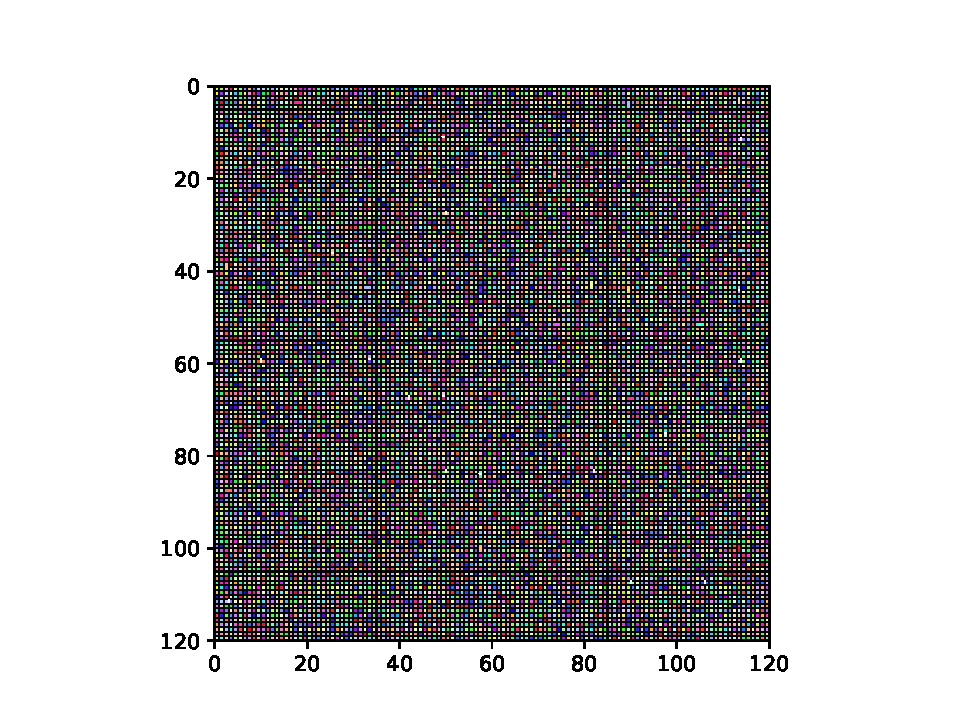
\includegraphics[width=\columnwidth,trim={2.5cm 0.5cm 2.5cm 1cm},clip]{img/ChannelMap_1011_update0}
  \caption{Update 0 (Generation 0)}
  \label{fig:ChannelMap_1011_update0}
\end{subfigure}%
\begin{subfigure}[b]{0.5\columnwidth}
  \includegraphics[width=\columnwidth,trim={2.5cm 0.5cm 2.5cm 1cm},clip]{img/ChannelMap_1011_update1000000}
  \caption{Update 1 million (Generation 927)}
  \label{fig:ChannelMap_1011_update1000000}
\end{subfigure}
\begin{subfigure}[b]{0.5\columnwidth}
  \includegraphics[width=\columnwidth,trim={2.5cm 0.5cm 2.5cm 1cm},clip]{img/ChannelMap_1011_update2000000}
  \caption{Update 2 million (Generation 1917)}
  \label{fig:ChannelMap_1011_update2000000}
\end{subfigure}%
\begin{subfigure}[b]{0.5\columnwidth}
  \includegraphics[width=\columnwidth,trim={2.5cm 0.5cm 2.5cm 1cm},clip]{img/ChannelMap_1011_update4000000}
  \caption{Update 4 million (Generation 4053)}
  \label{fig:ChannelMap_1011_update4000000}
\end{subfigure}
\begin{subfigure}[b]{0.5\columnwidth}
  \includegraphics[width=\columnwidth,trim={2.5cm 0.5cm 2.5cm 1cm},clip]{img/ChannelMap_1011_update5000000}
  \caption{Update 5 million (Generation 5173)}
  \label{fig:ChannelMap_1011_update5000000}
\end{subfigure}%
\begin{subfigure}[b]{0.5\columnwidth}
  \includegraphics[width=\columnwidth,trim={2.5cm 0.5cm 2.5cm 1cm},clip]{img/ChannelMap_1011_update7000000}
  \caption{Update 7 million (Generation 7312)}
  \label{fig:ChannelMap_1011_update7000000}
\end{subfigure}
\caption{
Progression of of same-channel level-zero and level-one signaling networks states in an evolutionary run where population mean $P_1 > P_{self}, P_0$ evolved.
Level-zero channels coded by HSV value are separated by white borders and level-one channels coded by HSV hue are separated by black borders.
}
\label{fig:grid_progression}
\end{center}
\end{figure}


\begin{figure}[t]
\begin{center}

\begin{subfigure}[b]{\columnwidth}
  \includegraphics[width=\columnwidth]{img/champion_res_pool1_vs_champion_damage_suicide0}
  \label{fig:champion_res_pool1_vs_champion_damage_suicide0}
\end{subfigure}

\begin{subfigure}[b]{\columnwidth}
  \includegraphics[width=\columnwidth]{img/champion_res_pool2_vs_champion_damage_suicide0}
  \label{fig:champion_res_pool2_vs_champion_damage_suicide0}
\end{subfigure}

\caption{
TODO
}
\label{fig:damage_suicide}
\end{center}
\end{figure}


\begin{figure}[!htbp]
\begin{center}

\begin{subfigure}[b]{0.5\columnwidth}
  \includegraphics[width=\columnwidth]{img/mean_res_pool1_vs_net_reproduction}
  \caption{
  Correlation plot of population mean $P_0$ and population net reproduction rate.
  }
  \label{fig:mean_res_pool1_vs_net_reproduction}
\end{subfigure}%
\begin{subfigure}[b]{0.5\columnwidth}
  \includegraphics[width=\columnwidth]{img/mean_res_pool2_vs_net_reproduction}
  \caption{
  Correlation plot of population mean $P_1$ and population net reproduction rate.
  }
  \label{fig:mean_res_pool2_vs_net_reproduction}
\end{subfigure}
\caption{
Mean resource caching strategies and net reproduction rate across populations.
A bootstrapped 95\% confidence interval for the fit is shaded.
}
\label{fig:net_reproduction}
\end{center}
\end{figure}


\begin{figure}[!htbp]
\begin{center}

\begin{subfigure}[b]{0.5\columnwidth}
  \includegraphics[width=\columnwidth]{img/champion_res_pool1_vs_champion_endowment2}
  \caption{
  Correlation plot of dominant genotype $P_1$ and dominant genotype $E_2$.
  }
  \label{fig:champion_res_pool1_vs_champion_endowment2}
\end{subfigure}%
\begin{subfigure}[b]{0.5\columnwidth}
  \includegraphics[width=\columnwidth]{img/champion_res_pool2_vs_champion_endowment2}
  \caption{
  Correlation plot of dominant genotype $P_2$ and dominant genotype $E_2$.
  }
  \label{fig:champion_res_pool2_vs_champion_endowment2}
\end{subfigure}

\caption{
Plots of dominant resource caching strategies and dominant propagule endowment strategies.
A bootstrapped 95\% confidence interval for the fit is shaded.
}
\label{fig:endowment}
\end{center}
\end{figure}


Zeroth-, first-, and second- level individuals were all observed at update 19.5 million (~ generation TODO) in different runs of our evolutionary simulation.
The criteria used to discern these outcomes are described below.
Figure \ref{fig:outcome_grids} shows the state of same-channel zero- and one-level signaling networks at the end of runs where zero-, first-, and second-level individuality evolved.
Figure \ref{fig:grid_progression} shows a series of signaling network snapshots in an evolutionary run where second-level individuality evolved.
Zeroth-level individuals appear to form with comparatively large zero-level signaling networks that are arranged into roughly globular one-level signaling networks.
First-level individuals appear to form elongated cigar-shaped one-level amalgamations of diversiform zero-level networks.
Second-level individuals appear to form highly regular diamond-shaped one- level amalgamations of diversiform zero-level networks.

Figure \ref{fig:genotypes} describes predominant genotypes observed at the end of evolutionary simulation.
With a single exception, nearly all evolved genotypes had $A_1$ fixed at or very near $1.0$ (i.e. population mean $A_1 \geq 0.993$) .
So, reproduction over cells sharing the same one-level channel was near-universally avoided;
genotypes evolved so that organisms located at the interior of one-level same-channel signaling networks surrendered their ability to reproduce (at least as long as they remained at the interior of the network).
We confirmed that reproductive abstention indeed occurred in our system as expected by directly logging it.

However, a variety of resource-caching strategies evolved.
Most-abundant genotypes at the end of evolutionary runs included strategies where resource was primarily cached in an organism's individual stockpile (i.e. $P_0 > P_1, P_2$), strategies where resource was primarily cached in an organism's zero-level signaling network's pool (i.e. $P_1 > P_0, P_2$), and strategies where resource was primarily cached in an organism's one-level signaling network's pool (i.e. $P_2 > P_0, P_1$).
Among 33 trials, at update $1.95 \times 10^{10}$ predominant genotypes with $P_0 > P_1, P_2$ were observed in two replicates, predominant genotypes with $P_1 > P_0, P_2$ were observed in 16 replicates, and predominant genotypes with $P_2 > P_0, P_1$ were observed in 15 replicates.
A related measure, among populations at update $1.999 \times 10^{10}$ mean $P_0 > P_1, P_2$ was observed in one replicate, mean $P_1 > P_0, P_2$ was observed in 16 replicates, and mean $P_2 > P_0, P_2$ was observed in 16 replicates.

Given the near-ubiquitous nature of cooperation with regard to reproductive division of labor at the one-level same-channel signaling network, it was on this basis of resource caching strategy that distinctions between zeroth-, first-, and second- level individuality was drawn.
(The single predominant genotype with $A_1 = 0.91$ had $P_1 = 1.0$, so was not sharing resource on the one-level same-channel resource pool).

Given that zeroth-, first-, and second-level individuals evolved, we wanted to set aside questions of evolutionary dynamics to determine which genotype was the most fit in the DISHTINY environment.
To accomplish this, we ran ecological competitions between the the dominant genotypes from the run with greatest mean $P_0$, the run with greatest mean $P_1$, and the run with greatest mean $P_2$.
Out of 191 trials performed, by update $1.5 \times 10^{10}$, fixation was reached.
The zeroth-level individuality genotype was predominant in one trial, the first-level individuality genotype was predominant in 12 trials, and the second-level individuality genotype was predominant in 178 trials.
These results suggest that in the absence of mutation, second-level individuals exhibits greater fitness than first- and zero-th level individuals ($p < 0.0001$; RR 2.8; two-tailed exact test).

In this comparison, however, higher-level individuality likely benefited from eliminated the problem of somatic mutation.
To assess the relative fitness of first- and second-level individuals without mutation disabled, we examined the relationship between mean $P_1$ and $P_2$ at update $1.95 \times 10^{10}$ and the rate of cellular reproduction at update $1.999 \times 10^{10}$ in the 33 replicate evolutionary trials performed.
We observed a significant negative correlation between mean $P_1$ and cellular reproduction rate ($p < 0.0001$; bootstrap test; Figure \ref{fig:mean_res_pool1_vs_net_reproduction}) and a significant positive correlation between mean $P_2$ and cellular reproduction rate was observed ($p < 0.0001$; bootstrap test; Figure \ref{fig:mean_res_pool2_vs_net_reproduction}).
This suggests that second-level individuals tend to collect resource more effectively than first-level individuals.
We did not test correlation between $P_0$ and due to the small number of outcomes where elevated $P_0$ was observed.

With the viability of zero-, first-, and second-level individuality in the DISHTINY environment --- and the greater relative fitness of second-level individuality --- established, we were also interested in probing the strategies employed by zero-, first-, and second-level individuals beyond resource caching and reproductive deferment.
To assess whether higher-level individuals employed apoptosis to mitigate somatic mutation, we examined the relationship between dominant genotype $P_1$ and $P_2$ and dominant genotype $M_0$ at update $1.95 \times 10^{10}$ in the 33 replicate evolutionary trials performed.
We observed a significant negative correlation between dominant genotype $P_1$ and $M_0$ ($p < 0.0001$; bootstrap test; Figure \ref{fig:champion_res_pool1_vs_champion_damage_suicide0}) and a significant positive correlation between dominant genotype $P_2$ and $M_0$ ($p < 0.0001$; bootstrap test; Figure \ref{fig:champion_res_pool2_vs_champion_damage_suicide0}).
Notably, no genotype encoding second-level individuality was observed with $M_0 < 0.5$.
This suggests that second-level individuals, in particular, relied on apoptosis to mitigate somatic mutation, perhaps due to their much larger scale compared to first- and zeroth-level individuals.

To assess whether higher-level individuals provided propagules (offspring sharing neither the zero- nor the one-level channel ID with the parent) with larger resource endowments, we examined the relationship between dominant genotype $P_1$ and $P_2$ and dominant genotype $E_2$ at update $1.95 \times 10^{10}$ in the 33 replicate evolutionary trials performed.
We observed a significant negative correlation between dominant genotype $P_1$ and $E_2$ ($p < 0.001$; bootstrap test; Figure \ref{fig:champion_res_pool1_vs_champion_endowment2}) and a significant positive correlation between dominant genotype $P_2$ and $E_2$ ($p <  0.0001$; bootstrap test; Figure \ref{fig:champion_res_pool2_vs_champion_endowment2}).
Second-level individuals might provide larger endowments to propagules simply due to a greater capacity to collect resource or perhaps because of stronger selection for well-endowed offspring when competing against other second-level individuals.
